\documentclass[type=dr, dr=rernat, accentcolor=tud7b,colorbacktitle, bigchapter, openright, twoside, 12pt ]{tudthesis}
%\documentclass[11pt,twoside,a4paper]{article}
\usepackage[english]{babel} 
\usepackage[utf8]{inputenc}
\usepackage{graphicx}
\usepackage{pstricks}
\usepackage{psfrag}
\usepackage{enumerate}
\usepackage{float}
\usepackage{epsfig}
\usepackage{geometry}
\usepackage{subfigure}
\usepackage{rotating}
\usepackage{minitoc}
%\usepackage{appendix}

%%%% 1 1/2 facher Zeilenabstand:	
\usepackage{setspace}
\onehalfspacing




\begin{document}
\chapter{Research background and Fundamentals}
\label{chapter:intro}
\minitoc

\section{Radiotherapy}

Since the discovery of X-rays in 1895 the radiation has been used by physicans for treating patients. 
In the begining only superfical diseases could be cured, but as time and technology progressed X-ray tubes gained on voltage
and allowing treatment of deeper suited tumors.

The radiation from linear accelerator was first used in medicine in 1953. Because the beam is more collimated and energies are
higher than X-ray tube the cure rates improved tremendously. The next big milestone was introduction of computeres in the field
of radiotherapy. This led to better diagnostic tools, such as computed tomography scans (CT), magnetic resonance imaging (MRI) and
positron emission tomography (PET). With those tools the location of the tumor could be much better estimated and hence the physicans
could easier prescribe treatment. The potential of computers were afterwards exploited also in treatment planning with intensity modulated
radiation therapy (IMRT) which, together with diagnostic tools, provides an exact dose shaping in accordance to patient specific tumors.

In 1946 it was discovered that protons could be used alongside photons for cancer treatment. Furthermore it was shown that protons have preferable depth dose profile 
compared to photons. First patient treatment soon followed in the early 1950's at Lawrence Berkeley Laboratory, USA. Heavier ions, such as 
He$^{2+}$, $^{20}$Ne and $^6$C were also used later on for treatment. In the begining only passive beam delivery was used for treatment 
and in the 1990's active beam solutions were developed at Paul Scherrer Institut (PSI), Villigen (Switzerland) for protons and at GSI, Darmstadt 
(Germany) for carbon ions.

Both treatment modalities (photons and ions) use the same principle to eliminate cancer cells. The physical and biological mechanism behind 
it will be explained in detail in the following sections.


\section{Physcial and biological basics of radiotherapy}

\subsection{Interaction of radiation with matter}

The interactions between photons and ions with matter are quite different, as can be seen from depth dose distributions in Figure \ref{ddp}.  Photons deposit highest local dose shortly after entering the matter 
(at the energies used in radiotherapy). Ions deposit most of their dose right before they stop in the Bragg Peak region. The position of the Bragg Peak depends on the energy of the ions, which is exploited in the treatment
of deep suited tumors.

\newpage
 
\vspace*{1cm}
 
\begin{figure}[H]
\begin{center}
% 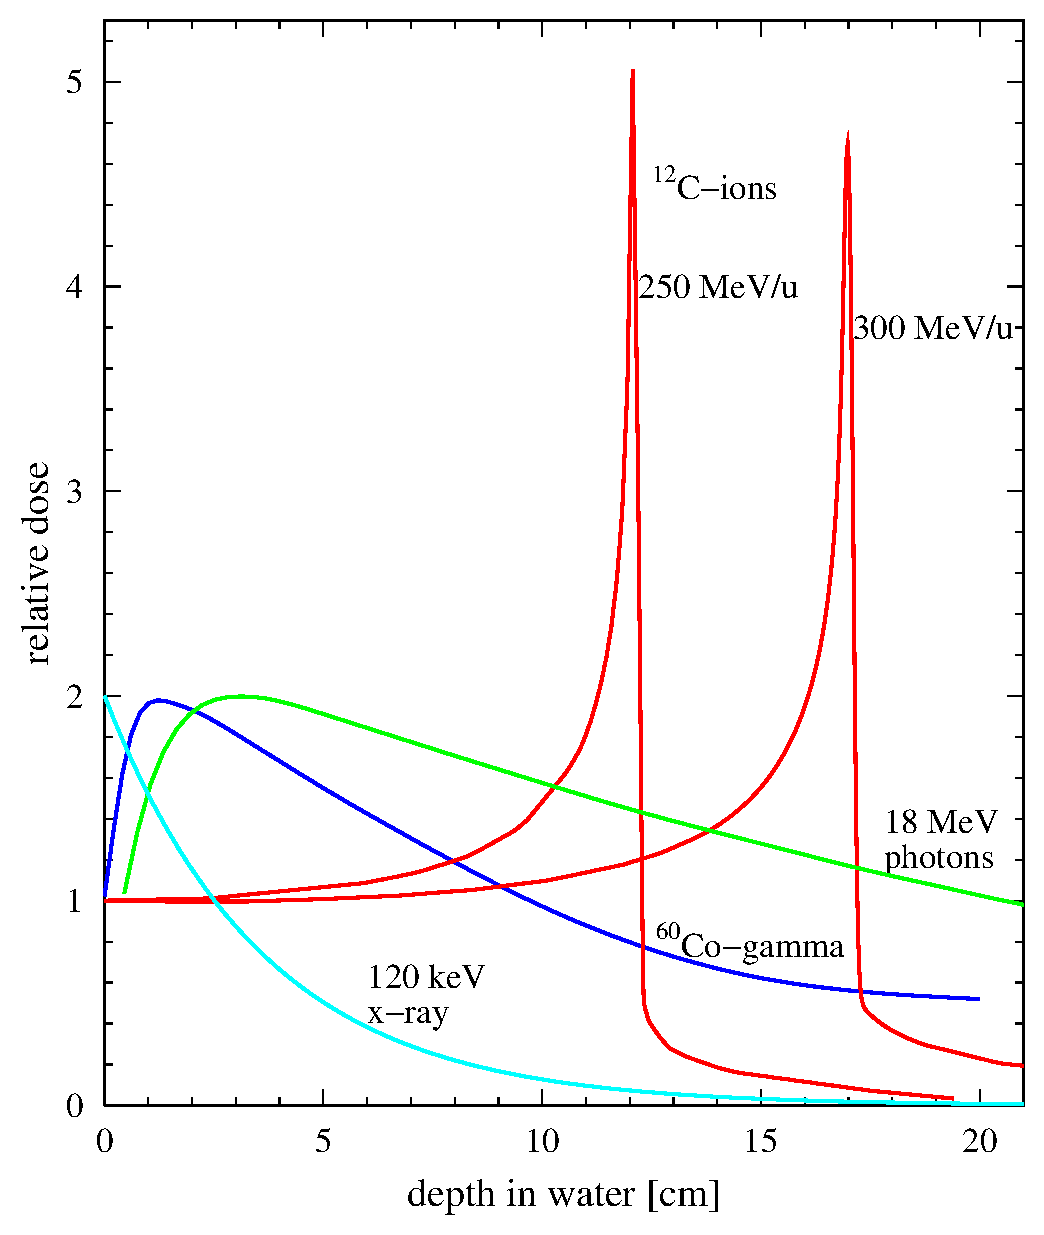
\includegraphics[scale=1]{depthdose.eps}
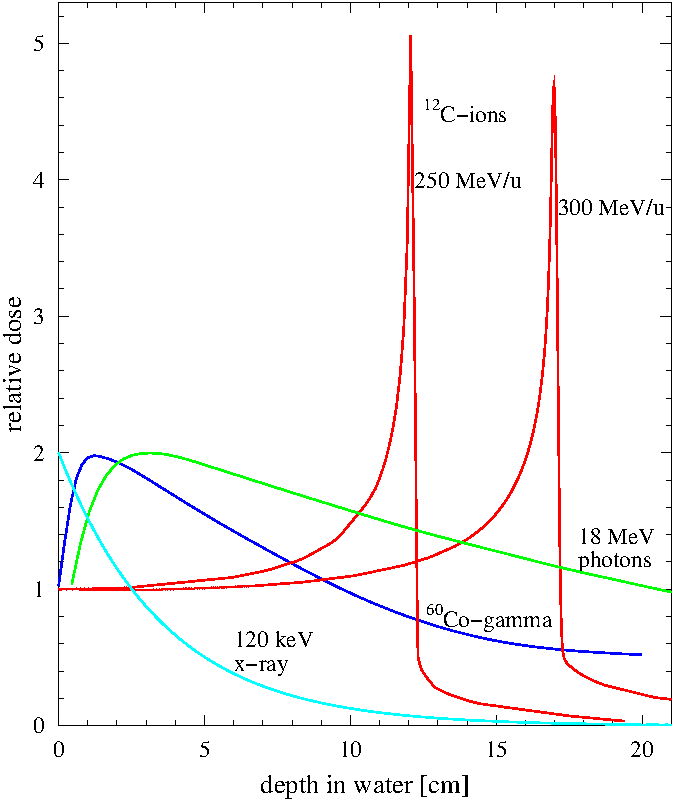
\includegraphics[scale=1]{./Images/depthdose.png}
\caption{Photon and carbon ions depth dose distributions at different energies. Photons start with a build up, which is followed by an exponential decrease after.
Ions deposit most of the dose at the end of the particle track, the Bragg peak. Figure taken from \cite{Schardt2010} }
\label{ddp}
\end{center}
\end{figure}

\subsection{Dose definition}

Physicis in radiotherapy revolves around dose, $D$, which is defined as the ratio of the absorbed energy $dE$ per mass element $dm$ \cite{ICRU1993}:

\begin{equation}
 D = \frac{dE}{dm}
\end{equation}

Usually we can describe energy loss of a beam in a thin layer of material, $dE/dx$. Dose can be then rewritten as:

\begin{equation}
 D = \frac{dE}{dx} \times \frac{1}{F} \times \frac{1}{\rho}
\end{equation}

where $F$ is fluence and $\rho$ the material denisty.



\subsubsection{Interaction of photons with matter}

Photons mostly interact with matter in one of the following ways: coherent or Rayleigh scattering, photoelectric effect, Compton scattering and pair production. The cross section, $\sigma$, for each of these processes depends
as well on the energy of the indicent photons as on the atomic number of the absorbin material \cite{Lilley2006}. The decreasing photon intesity in matter, $I$, can be described as:


\begin{equation}
 I = I_{0} \cdot e^{- N \sigma x} = I_{0} \cdot e^{-\mu x}
 \label{expdecrease}
\end{equation} 

where $I_{0}$ stands for the initial intensity of the photons, $x$ the depth of the material in units of length, $N$ the atomic density of the material and $\mu$ is the attenuation coefficient. The cross section, $sigma$ is the sum of all
possibile Interaction processes.

\begin{equation}
{\sigma} = \sigma_{rayleigh} + \sigma_{photoelectric} + Z\sigma_{compton} + \sigma_{pairproduction} 
\end{equation}

The energy range of photons used in radiotherapy is between 100 keV and 25 MeV. The dominating process in this energy range is Compton scattering \cite{Alpen1998}.
The electrons resulting from Compton interaction scatter mostly in a forward direction. Therefore a maximum of the depth-dose profile occurs when electrons stop at a certain depth, 
the mean electron range. After this build up the dose deposition decreases exponentially (see Figure \ref{ddp} and Equation \ref{expdecrease}).


\subsubsection{Interaction of ions with matter}
\label{iion}
Ions can interact with matter either with elastic columb scattering from target nuclei (nuclear stopping) or with inelastic collision with target electorns (electronic stopping).
At the ion energies used in radiotherapy, which are less then 500$\mathrm{MeV}/\mathrm{u}$, the electronic stoping is the dominated interaction. This results in ionization and excitation of the atoms in target.

The mean rate of ions energy loss in matter is described by the Bethe-Bloch formula \cite{Bethe1930, Bloch1933}. Since we are interested in low ion energies, we can make the following approximation:

\begin{equation}
- \left \langle \frac{dE}{dx} \right \rangle = \frac{ 4 \pi N_{e} z_{eff}^{2} }{ m_{e} v^{2} } \left( \frac{e^{2}}{4\pi \epsilon_{0}} \right) ^{2} \left[ln \left( \frac{2m_{e}v^{2}}{I} \right)+correction \right]
 \label{bethe}
\end{equation}

here $N_{e}$ is the materials electron density, $e$ and $m_{e}$ are the charge and mass 
of an electron, $\epsilon_{0}$ the electrical field constant and $I$ the mean excitation energy of the absorber material. 
Barkas formula \cite{Barkas1963} can be used for the approximation of the effective projectile charge $z_{eff}$: 

% \vspace*{-0.8cm}
\begin{equation}
 z_{eff} = z \left( 1 - e^{-125 \beta z^{\frac{2}{3}}} \right)
\end{equation}

where $\beta$ is the projectile speed in units of $c$.

The energy loss of ions is proportional to $z_{eff}$ and inversely proportional to $v^2$. The shape of the curve in Figure \ref{ddp} can now be understood. Ions enter the matter with a high velocity,
resulting in a small energy deposition. Their velocity gradualy decreases, which in turn increases the energy deposition. The maximum of the energy loss is called Bragg peak or particle range.

\subsubsection{Lateral scattering and range straggling of ions}
\label{scat}
As mentioned in section \ref{iion} ions interact mostly via electronic stopping at energies used in radiotherapy. However, nuclear stopping still occurs and it is the main reason for lateral scattering.
The angular spread of ions is dependent on the mass of the target nuclei and on the momentum of the indecient ions \cite{Moliere1948}. The lateral scattering is proportional to mass of the target nuclei and inversely proportional
on the momentum of indecient ions. Carbon ions have thus less lateral scatter then protons. Experiments have shown that carbon ions have three times smaller angular spread compared to protons at the same range in water 
(15.6 cm, 150 MeV/u protons and 285 MeV/u $^{12}$C ions) \cite{Schardt2010}.

Statistical fluctuations of specific electronic stopping events cause range straggling of ions. If the number of collisions is high or the material is thick enoguh these fluctuations can be approximated by
a Gaussian probability distribution \cite{Bohr1940, Ahlen1980}. The straggling width $\sigma_R$ is proportional to:

\begin{equation}
 \sigma_R \propto R/\sqrt{M}
\end{equation}

where $R$ is the mean range of ions and $M$ the ion mass. Thus, the heavier the ion is, the less range straggling it has. Carbon ions have 3.5 smaller range straggling when compared to protons \cite{Schardt2010}.

\subsubsection{Nuclear fragmentation}
\label{nuclfrag}

When transversing through matter ions (except protons) can be fragmented into ions with lower Z. The lower Z fragments travel in the same direction as projectile ions and 
have a significant contribution to the dose deposited (see Figure \ref{iondd}). It is essential that this fragments are included in the treatment planning, so that the accurate dose can be assesed.

After colliding with target projectile fragments enter in a excited state. De-excitation occurs through
emisson of nucleons, nucleon clusters and photons. Two of the possible fragments of projectile $^{12}$C ions are isotopes $^{11}C$ and $^{10}C$, which are both $\beta^+$ emmiters \cite{Kraft2000}.
The resulting positron is annihilated with electrons in matter, resulting in two photons traveling in opposite direction. This can be used in PET (Positron Emission Tomography) without exposing patient
to additional radiation.. 

\begin{figure}[H]
\begin{center}
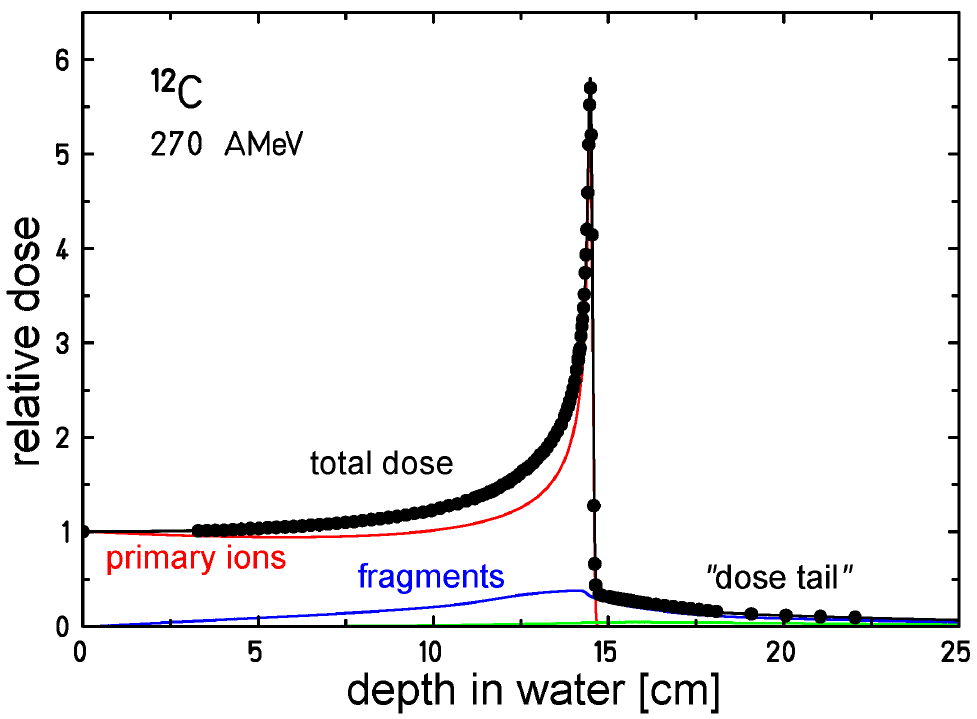
\includegraphics[scale=0.3]{./Images/iondepthdosesum.png}
\caption{Impact of fragmantation on a depth dose distribution of carbon ions. Main contribution to the overall deposited dose (black line) comes from the primary ions (red line). The produced fragments 
(blue line) have a smaller impact, but non-negleigble especially in the dose tail behind the Bragg peak. Figure taken from \cite{Groezinger2004}}
\label{iondd}
\end{center}
\end{figure}

\subsubsection{Secondary electrons and track structure}

As mentioned in section \ref{iion} ions used in radiotherapy lose most of their energy via inelastic Coulumb scattering on target electrons. Such electrons can be libirated from target atoms and are called
secondary electrons, also $\delta$-electrons. $\delta$-electrons also travel throguh matter, further scattering and may even cause secondary ionization of the target atoms. When $\delta$-electrons energies are larger than $>$50 eV,
ionization becomes dominant process, which produces a large number of additional electrons \cite{Kraft2000,Schardt2010}.

The radial dose profile and track diameter is defined by the energy spectrum of the $\delta$-electrons. Most of the $\delta$-electorns are concentrated around the projectile ions path, since they receive small energy transfers 
or are scattered in the direction of indicent ions. Different models \cite{!!}, Monte Carlo simulations \cite{!!} predict radial dose fall-off approximatelly with $1/r^2$ for radial distances $r$. Varma et. al. have confirmed 
this experimentaly \cite{Varma1977}. The maximum radial distance $r_{max}$ is defined by the most energetic $\delta$-electrons, which are related to energy, $E$, of the projectile ions \cite{Kiefer1986}.

\begin{equation}
 r_{max} = E^{1.7}
\end{equation}

Following equation \ref{bethe}, $E$ is corelated to $Z^2$ and $1/\beta^2$, which means track structure is highly dependent on the projectile ion species and energy. This is well demonstrated on Figure \ref{track}:
Carbon ions have much more dense ionization structure compared to protons \cite{!!}. $\delta$-electrons have low energies, and thus the $r$ is on nanometer scale. As the energy of projectile ions decreases, their
stopping power increases and causes significantly larger number of $\delta$-electorns. The energy deposited by $\delta$-electrons in medium is described using the Linear Energy Transfer (LET), which is closely related to 
$dE/dx$. Fast ions, with little ionization, have thus small LET, while slow ions, with large ionization, have a high LET.


\begin{figure}[H]
\begin{center}
% 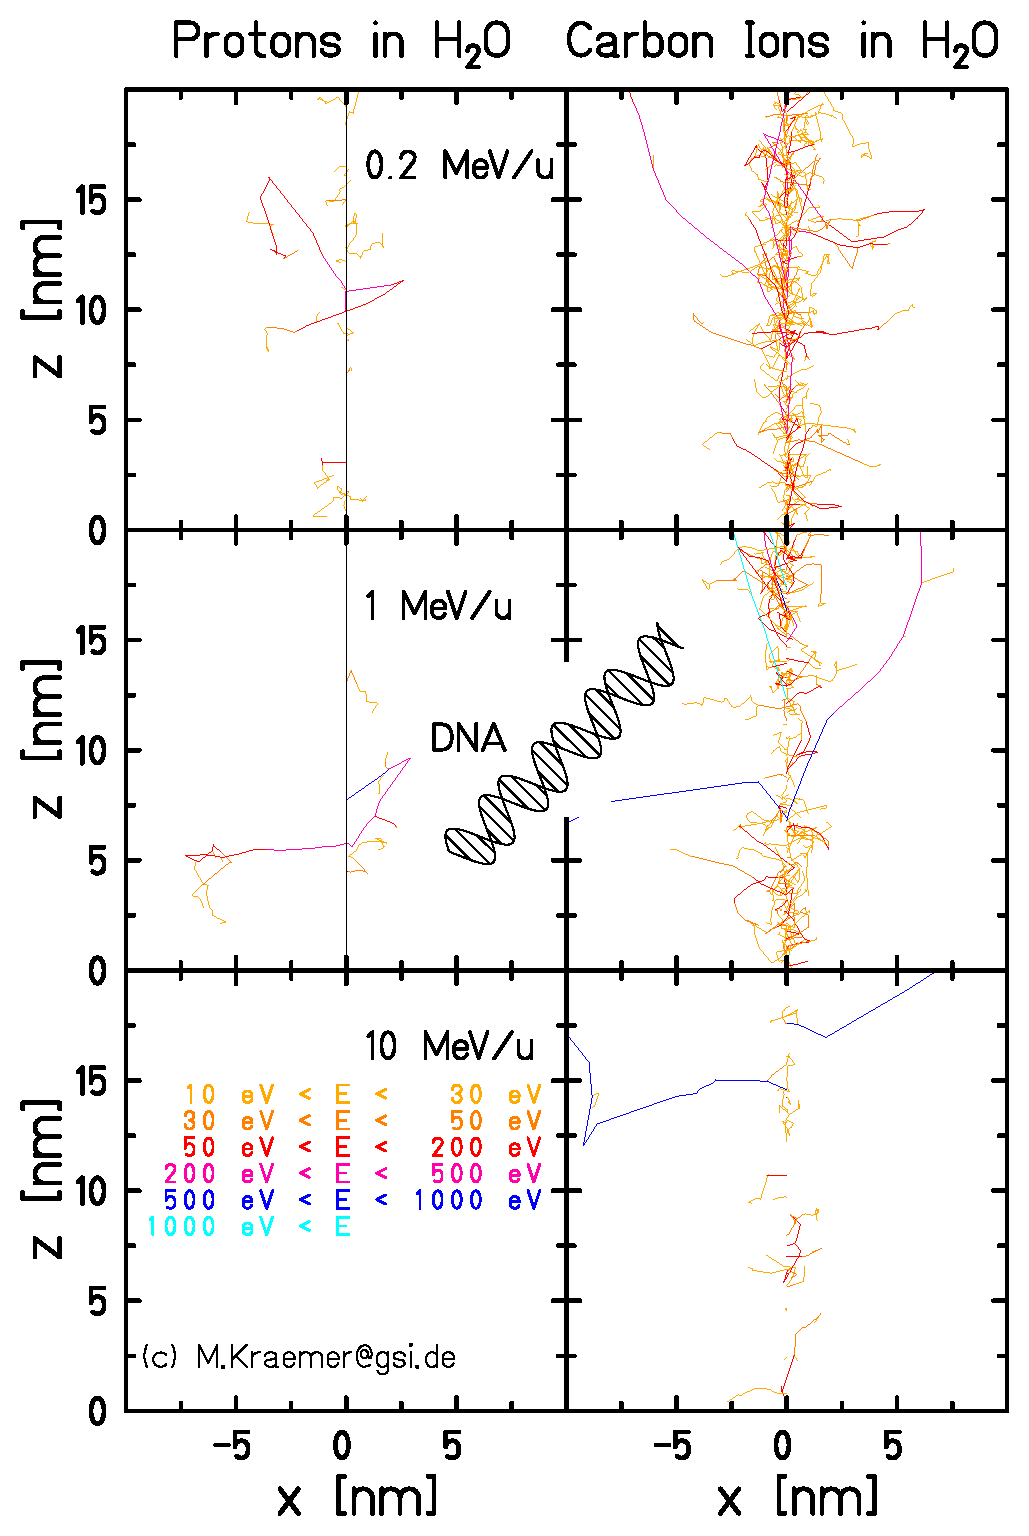
\includegraphics[scale=0.75]{trackstructure.eps}
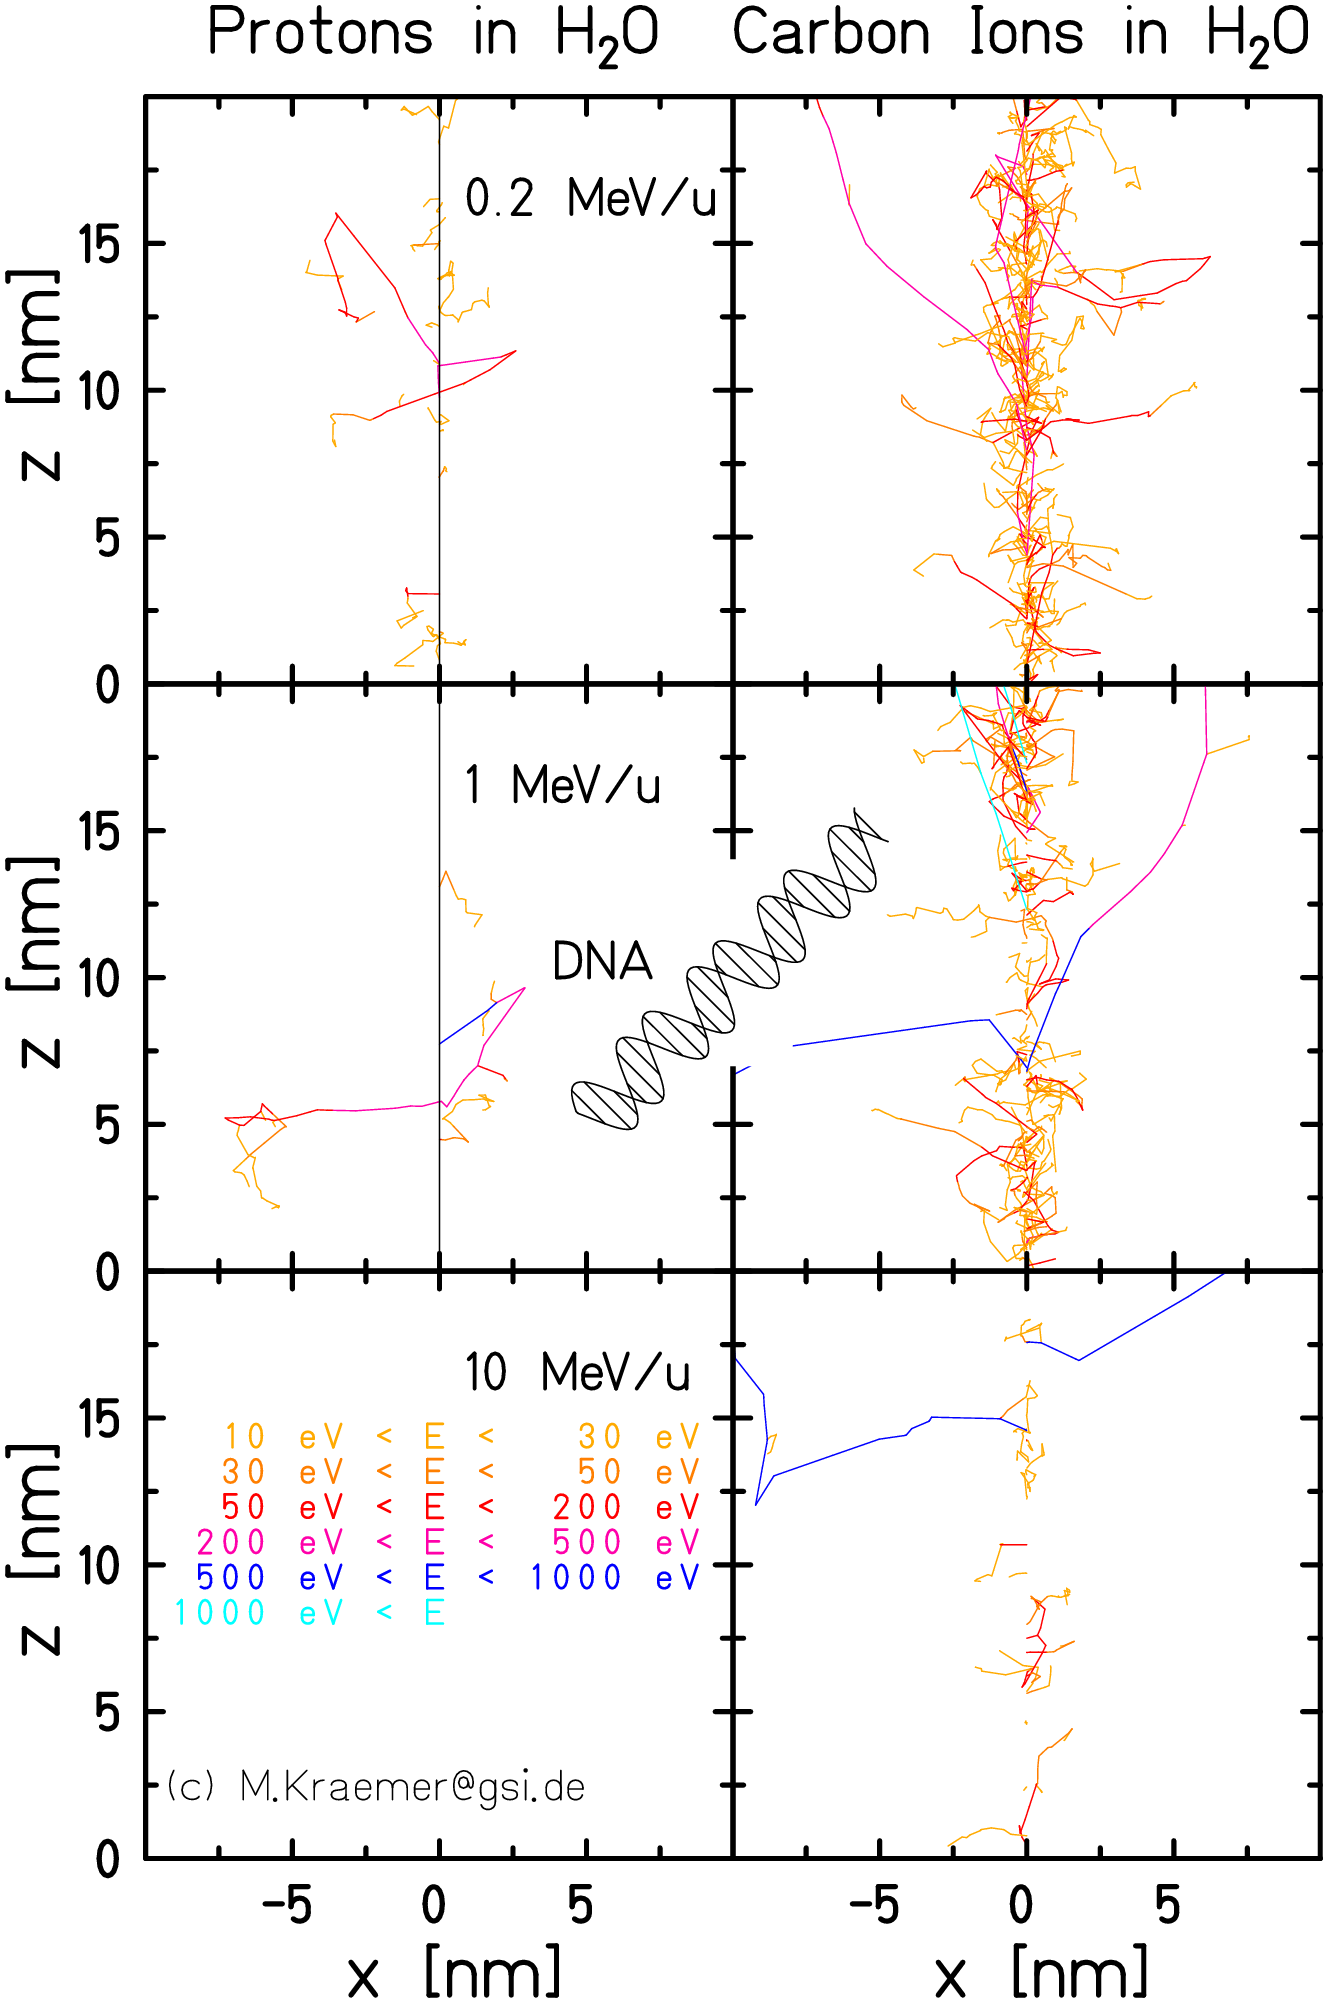
\includegraphics[scale=0.25]{./Images/trackstructure.png}
\caption{Track structure of ions in water at different energies. The distribution of $\delta$-electrons is highly dependent on ion species and their energy.
A molecule of DNA is displayed for size comparison. Figure courtesy of Michael Kr\"amer.}
\label{track}
\end{center}
\end{figure}


\subsection{Radiobiology}

The aim of radiotherapy is to kill tumor cells and prevent furhter growth, while sparring healthy tissue. Ionizing radiation (photons and ions) causes damage throughout the cell. However the most susceptible part to radiation is the
carrier of genetic information, the deoxyribonucleic acid (DNA), located in the cell nucleus \cite{Munro1970}. Radiation can destroy DNA in two ways - directly or inderectly. Ionization and consequent destruction of DNA molecular bonds
via radiation is a direct effect (see Figure \ref{ida}b) and is typical for high-LET radiation. On the other hand, an indirect effect is when radiation hydrolyses water around DNA and produce highly reactive hydroxyl-radicals, OH 
(see Figure \ref{ida}a). Eventhough their lifetime is short, it's enough to cause severe damage to DNA. The formation of OH is typical for low-LET radiation, like photons. The two processes, direct and inderect, are not 
excluding and can damage DNA in parallel.

Damage to DNA can result in either single strand breaks (SSB) or double strand breaks (DSB) as  shown in Figure \ref{ida}b). When one of the double strands in the DNA helix is destroyed (SSB), it can be usually easily repaired by cell 
repair-mechanisms, since the complementary base is intact. If bases on both stands are destroyed (DSB) the DNA damage is much more complex and can lead to the breakage of the chromatin. The cell repair-mechanisms can handle DSB as well, 
albeit not that efficient as SSB. However if there are clustered DSBs, the damage is usually too severe for repair-mechanisms to undo it. The changes in damaged DNA can lead to carcinogenesis or cell death. The aim of radiotherapy is to 
cause apoptosis - a controlled self-inactivation of the cell due to DNA damage. Beside apoptosis, there is necrosis, an uncontrolled cell death. Cell necrosis often cause response from the immune system, leading to inflammation, which
radiotherapy tends to avoid.

\begin{figure}[H]
\begin{center}
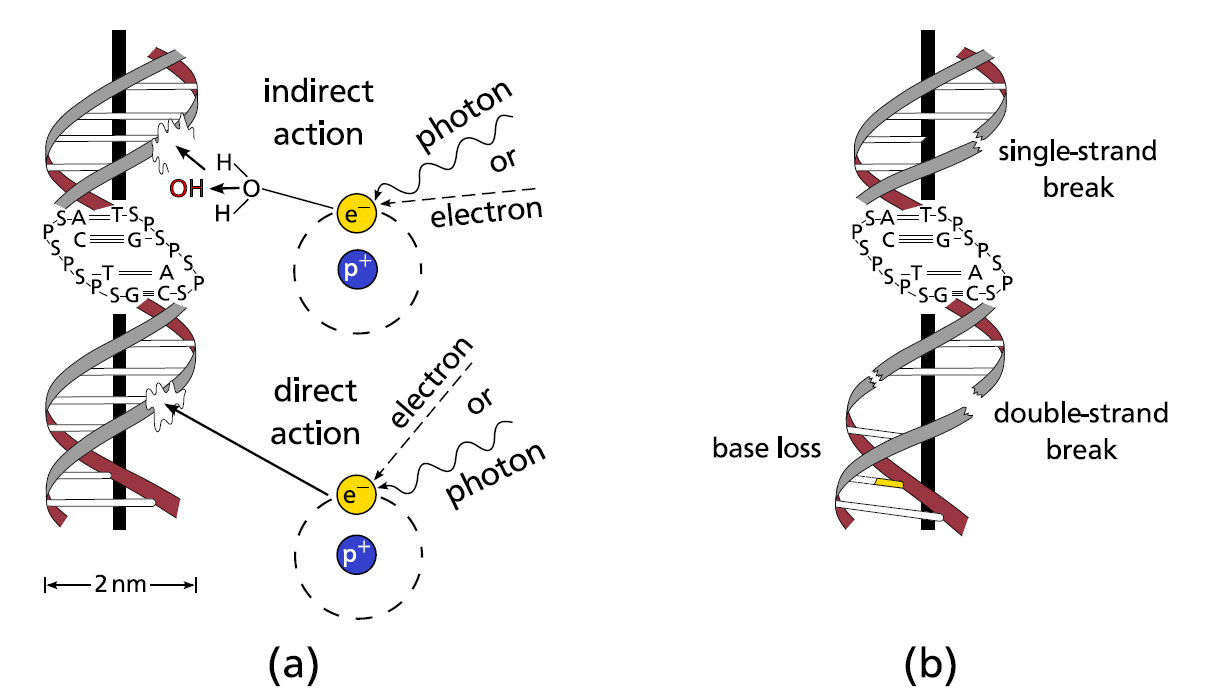
\includegraphics[scale=0.5]{SSB_DSB.png}
\caption{Types of DNA damage caused by radiadtion. (a) Indirect damage occurs, when radiation forms free radicals hydroxyl radicals (OH), which can damage DNA. (b) Direct effects of radiation can cause single or double-strand breaks. 
Figure taken from \cite{Richter2012}}
\label{ida}
\end{center}
\end{figure}


\subsubsection{Relative Biological Effectiveness}

Figure \ref{track} shows the size of DNA molecule in comparison with proton and carbon ion distribution of $\delta$-electrons around their track. Clustered DSB occur around ions Bragg peak due to the large ionization denseties. As mentioned
this poses a too large of a dificulty for cell repair-mechanisms, leading to cell death. The large ionization density is typical for ions and is one of the main advantages over photons in radiotherapeutic sense. Since most of the research about
cell response to radiadtion was done for photons, the biological effect of ions is usually described relative to a reference photon response. Relative biological effectiveness (RBE) is therefore defined as the ratio of the reference 
photon dose to the dose level of a specific ion radiation at the same biological effect (isoeffect):

\begin{equation}
 RBE = \left.\frac{D^{ref}_{photon}}{D_{ion}} \right|_{isoeffect}
\end{equation}



\bibliographystyle{apalike}
\bibliography{../ref.bib}{}
% \bibliographystyle{plain}

\end{document}